\subsection{Direzioni emergenti per l'elaborazione serverless sostenibile}
\label{subsec:direzioni_sostenibili}

Oltre agli interventi infrastrutturali descritti in precedenza, lo stato
dell'arte evidenzia direzioni complementari volte a rendere l'esecuzione
serverless più sostenibile attraverso meccanismi che agiscono a livello
applicativo piuttosto che infrastrutturale. Anziché intervenire sulla
distribuzione del carico o sulla potenza erogata ai nodi, tali approcci
modificano la relazione tra il comportamento dell'applicazione e il
consumo energetico, introducendo forme di controllo più fine.

Una prima direzione è rappresentata dal paradigma
dell'\emph{Approximate Computing}, che consente di ridurre il consumo
energetico accettando, in modo controllato, una diminuzione
dell'accuratezza del risultato. In questo ambito si colloca
JouleGuard~\cite{jouleguard}, che propone un modello di controllo runtime
capace di rispettare un budget energetico prefissato regolando
dinamicamente il livello di accuratezza dell'applicazione.

\begin{figure}[htbp]
    \centering
    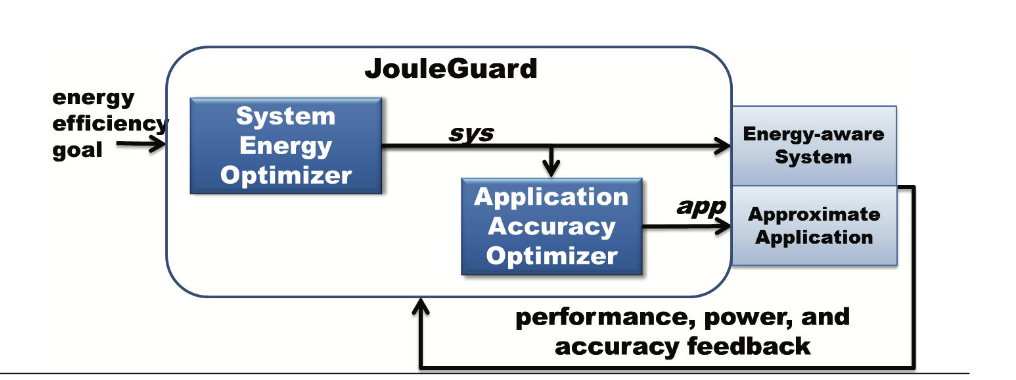
\includegraphics[width=0.8\textwidth]{figures/Jouleguard.png}
    \caption{Schema concettuale di JouleGuard. Il sistema regola
    dinamicamente il livello di accuratezza dell'applicazione in funzione
    di un vincolo energetico esplicito, trattando il budget di potenza
    come parametro attivo nel processo di controllo.}
    \label{fig:jouleguard}
\end{figure}

Come illustrato in Figura~\ref{fig:jouleguard}, il tratto distintivo di
JouleGuard consiste nel trattare l'energia non come una metrica da
minimizzare, ma come un vincolo esplicito che guida il comportamento del
sistema a runtime. La selezione del livello di approssimazione non è
determinata staticamente, ma dipende dalle condizioni operative osservate,
rendendo il sistema adattivo rispetto alla disponibilità energetica
corrente.

Una seconda direzione emerge dal lavoro \emph{Code Once, Run
Green}~\cite{refaas}, che propone di intervenire sull'implementazione
delle funzioni serverless mantenendone invariata la semantica. Gli autori
considerano la medesima funzione logica e ne realizzano una traduzione
automatica verso un linguaggio di programmazione differente,
consentendone l'esecuzione su runtime alternativi con potenziali profili
energetici più favorevoli.

\begin{figure}[htbp]
    \centering
    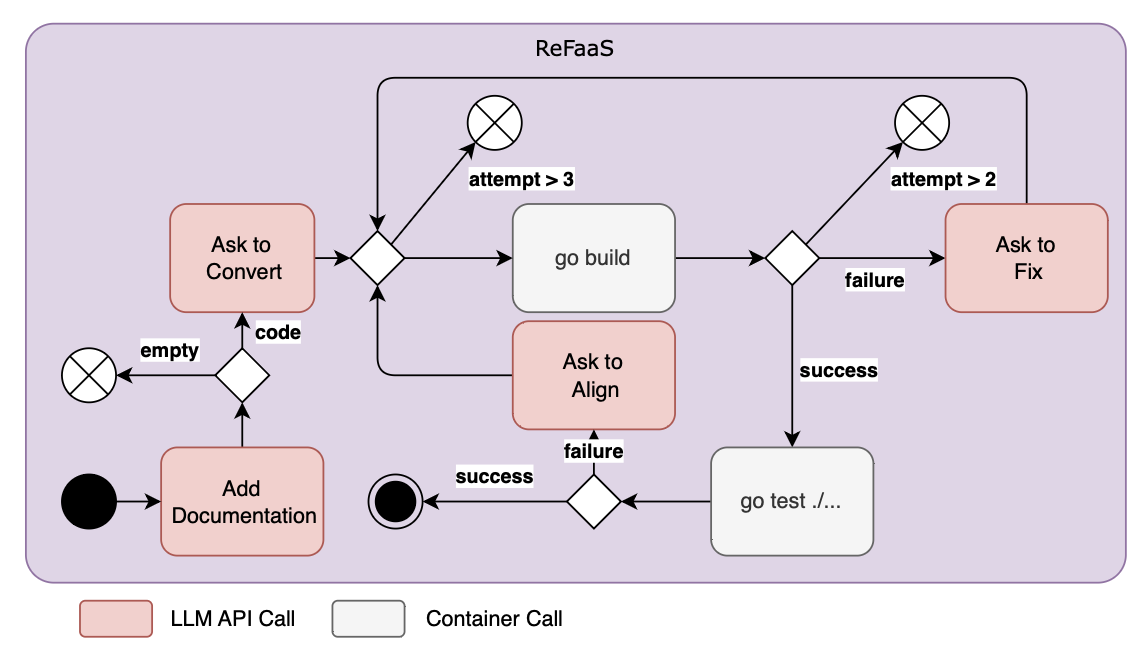
\includegraphics[width=0.85\textwidth]{figures/refaas.png}
    \caption{Pipeline di traduzione automatica proposta in \emph{Code Once,
    Run Green}. La trasformazione avviene in fase di build tramite un
    processo iterativo di conversione e validazione del
    codice.}
    \label{fig:refaas_pipeline}
\end{figure}

Come mostrato in Figura~\ref{fig:refaas_pipeline}, la trasformazione del
codice avviene in fase di build tramite una pipeline di conversione e
validazione iterativa. A differenza dell'approccio di JouleGuard,
l'ottimizzazione energetica è qui perseguita staticamente, agendo sulla
scelta del runtime piuttosto che sul comportamento dell'applicazione
durante l'esecuzione. L'approccio introduce un costo energetico iniziale
associato alla traduzione, potenzialmente ammortizzabile nel tempo
attraverso la riduzione del consumo per invocazione della funzione
tradotta.

Nel loro insieme, i lavori esaminati mostrano come la sostenibilità
dell'elaborazione serverless possa essere perseguita anche al di fuori
degli interventi infrastrutturali, attraverso meccanismi che agiscono
sulla logica applicativa. JouleGuard introduce il concetto di vincolo
energetico esplicito come parametro attivo nel controllo runtime;
\emph{Code Once, Run Green} mostra come la generazione di varianti della
stessa funzione, eseguite su runtime differenti, possa produrre profili
energetici significativamente diversi a parità di semantica.